\documentclass[10pt,a4paper]{article}
\usepackage[utf8]{inputenc}
\usepackage[T1]{fontenc}
\usepackage[english]{babel}
\usepackage{geometry}
\usepackage{booktabs}
\usepackage{tabularx}
\usepackage{amsmath,amssymb}
\usepackage{graphicx}
\usepackage{hyperref}
\usepackage{microtype}
\usepackage{xcolor}
\usepackage{colortbl}
\usepackage{enumitem}
\usepackage{fancyhdr}
\usepackage{makecell}
\usepackage{siunitx}

\geometry{left=18mm,right=18mm,top=22mm,bottom=22mm}
\pagestyle{fancy}
\fancyhf{}
\rhead{\footnotesize Research Paper: Small Language Models Under Severe Resource Constraints}
\lhead{\footnotesize Independent Systems Engineering \& Applied Machine Learning}
\rfoot{\footnotesize Page \thepage}

\hypersetup{
    colorlinks=true,
    linkcolor=blue!70!black,
    citecolor=blue!70!black,
    urlcolor=blue!70!black
}

\newcolumntype{C}{>{\centering\arraybackslash}X}
\newcolumntype{L}[1]{>{\raggedright\arraybackslash}p{#1}}

\title{\textbf{\LARGE Reproducible Evaluation of Small Language Models Under Severe Memory and Compute Constraints}\\[0.4em]
\large Architectural Dynamics, Quantization Frontiers, Speculative Decoding, and Adversarial Vulnerabilities on a Reference Edge Testbed}
\author{\textbf{Anderson Tavares} \\ Department of Systems Engineering and Applied Machine Learning \\ Independent Systems Research Group \\ \url{https://github.com/AndersonTavares0/llm-research-bench}}
\date{October 24, 2026}

\begin{document}

\maketitle

\begin{abstract}
Deploying Small Language Models (SLMs, 2B--4B parameters) directly on physical edge devices delivers strict data sovereignty, deterministic execution latency, and zero external network egress. However, operating within severe physical memory limits ($\le 4096$\,MiB VRAM) introduces non-linear trade-offs between tensor quantization precision, autoregressive memory bandwidth, speculative execution, and adversarial robustness. This research presents a rigorous, reproducible empirical evaluation conducted on an NVIDIA GeForce GTX 1050 Ti GPU (4096\,MiB GDDR5, 128-bit bus, $112.0\text{ GB/s}$ theoretical bandwidth, 75W TDP, Compute Capability 6.1) as a reference edge testbed. We formally deconstruct every underlying architectural concept---including the Roofline model, arithmetic intensity, Key-Value (KV) cache analytical scaling, Multi-Token Prediction (MTP) speculative decoding, Model Context Protocol (MCP), and inferential statistical testing---prior to presenting empirical findings. Four candidate architectures (\textbf{Gemma-4-E2B-it}, \textbf{Qwen-3.5-4B}, \textbf{Qwen-3.5-2B}, and \textbf{Llama-3.2-3B}) were benchmarked under the \texttt{llama-server} runtime (commit b4120+) with continuous asynchronous NVML hardware telemetry sampled at 250\,ms intervals. A controlled Multi-Token Prediction ablation with $N=15$ repetitions isolated a statistically significant \textbf{30.9\%} overall throughput gain ($42.21 \pm 5.99$ vs $32.25 \pm 3.23$\,tok/s, 95\% Student's t CI, Welch's $t=3.139$, two-tailed $p=0.0049$, one-tailed $p=0.0024$, Cohen's $d=1.146$) and \textbf{33.2\%} in steady-state warmed execution ($44.95$ vs $33.75$\,tok/s, Welch's $t=19.38$, $p=1.67\times 10^{-11}$, Cohen's $d=7.32$), operating at 2038\,MiB VRAM. Controlled quantization comparison of Gemma-4-E2B demonstrated that non-uniform importance matrix quantization with MTP speculative decoding (IQ4\_XS) delivers a \textbf{59.2\% compound throughput advantage} over standard block quantization without MTP (Q4\_K\_M) in steady-state ($41.92$ vs $26.34$\,tok/s, Welch's $t=27.20$, $p=5.15\times 10^{-7}$, $\nu = 5.43$), of which approximately +19.6\% is attributable to pure tensor compression and the remainder to speculative draft acceleration. In exploratory adversarial safety evaluations ($N=6$), all models exhibited 100\% clean refusal across 5 direct exploit and persona jailbreak vectors, but universally succumbed (0\% resistance) to an indirect prompt injection embedded in system logs, demonstrating an architectural deficiency in current post-training alignment across untrusted context tokens.
\end{abstract}

\vspace{0.6em}
\noindent\textbf{Keywords:} Small Language Models, Memory-Constrained Systems, Roofline Model, Key-Value Cache, Speculative Decoding, Multi-Token Prediction, Model Context Protocol, NVML Telemetry, Inferential Statistics, Indirect Prompt Injection.

\section{Introduction and Research Problem}

Edge computing increasingly demands that autonomous inference, local controllers, and agentic workflows execute on physical on-premises hardware. Offloading inference to commercial cloud APIs compromises data privacy, introduces non-deterministic network latency, incurs continuous financial costs, and creates catastrophic failure modes during network partitions.

Small Language Models (SLMs) spanning 2 billion to 4 billion parameters have emerged as viable local engines capable of complex instruction following, code generation, and structured tool interaction. However, hosting these models on entry-level or legacy GPUs---specifically consumer accelerators constrained to $4096\text{ MiB}$ of VRAM such as the NVIDIA GeForce GTX 1050 Ti---imposes harsh physical boundaries.

Every generated token requires streaming billions of parameters across a memory bus limited to $112.0\text{ GB/s}$. Expanding the context window causes Key-Value (KV) cache allocations to compete directly with model weights for physical address space. Furthermore, aggressive quantization schemes designed to compress weight tensors can degrade multi-step quantitative reasoning or undermine agentic reliability.

\subsection{Research Questions and Hypotheses}
This investigation is guided by four formal Research Questions (RQs):
\begin{enumerate}[leftmargin=2.2em]
    \item \textbf{RQ1 (Speculative Decoding and Bandwidth Amortization):} To what extent does Multi-Token Prediction (MTP) speculative decoding mitigate the memory bandwidth bottleneck in compact models ($<3\text{B}$) on memory-bound hardware without dedicated draft models?
    \begin{itemize}[leftmargin=1.5em]
        \item \emph{Hypothesis $H_1$:} Reusing latent transformer representations via auxiliary linear prediction heads achieves a statistically significant throughput speedup ($S \ge 1.25\times, p < 0.01$, Cohen's $d > 0.8$) without increasing VRAM consumption.
        \item \emph{Null Hypothesis $H_0$:} Verification overhead and rejection cycles neutralize speculative gains ($\mu_{\text{MTP}} \le \mu_{\text{Base}}$).
    \end{itemize}
    \item \textbf{RQ2 (Quantization Frontiers and Microarchitectural Penalties):} How do non-uniform importance matrix quantizations (\texttt{IQ4\_XS}) compare against standard block quantizations (\texttt{Q4\_K\_M}) regarding memory bus saturation and decode throughput on architectures lacking native INT4 hardware acceleration?
    \item \textbf{RQ3 (Key-Value Cache Scaling and OOM Boundaries):} What are the analytical and empirical memory boundaries for context scaling ($L \in [256, 32768]$) under a strict $4096\text{ MiB}$ physical limit, and at what sequence lengths does cache quantization become strictly mandatory?
    \item \textbf{RQ4 (Adversarial Robustness and Agentic Boundary Isolation):} Do compact parameter budgets create an asymmetry between direct attack refusal (jailbreaks, exploit generation) and indirect context-borne prompt injections through external tools (Model Context Protocol)?
\end{enumerate}

\subsection{Experimental Variables, Baselines, and Controls}
\begin{itemize}[leftmargin=1.8em]
    \item \textbf{Independent Variables:} Model architecture (Gemma-4-E2B, Qwen-3.5-2B, Llama-3.2-3B, Qwen-3.5-4B), quantization format (\texttt{IQ4\_XS}, \texttt{Q4\_K\_M}, \texttt{Q4\_K\_XL}), decoding strategy (Base autoregressive vs.\ MTP speculative), and context sequence length ($L$).
    \item \textbf{Dependent Variables:} Autoregressive decode throughput ($\text{tok/s}$), Time To First Token ($\text{TTFT}$, $\text{ms}$), peak physical VRAM ($\text{MiB}$), continuous energy efficiency ($\text{tok/J}$), Attack Success Rate ($\text{ASR}$, \%), and tool schema compliance (\%).
    \item \textbf{Controlled Variables:} Fixed ambient thermal environment ($24^\circ\text{C}$), fan profile pinned at 100\%, deterministic greedy decoding ($\tau = 0.0$), seed determinism, and isolated Linux container execution without graphical display overhead.
    \item \textbf{Baselines:} Unquantized FP16 KV cache allocation; Gemma-4-E2B without MTP draft head; and benign system control queries for false-positive safety assessment.
\end{itemize}

\subsection{Reference Edge Hardware Testbed}
The NVIDIA GeForce GTX 1050 Ti (4096\,MiB GDDR5, GP107, Pascal microarchitecture, Compute 6.1) was selected as a \textbf{reference empirical edge testbed}. Featuring a 128-bit memory bus ($112.0\text{ GB/s}$) and lacking modern mixed-precision Tensor Cores, this accelerator represents the lower hardware boundary for local SLM deployment. Its constrained memory bandwidth exposes memory-bound bottlenecks and allows rigorous validation of whether software innovations (speculative decoding, importance quantization) can bridge hardware generation gaps.

\subsection{Paper Structure}
This paper is organized progressively: Section~2 establishes the theoretical foundations and didactic deconstructions. Section~3 defines benchmark suites and experimental controls. Section~4 analyzes system performance and telemetry. Section~5 presents controlled ablations and inferential statistical testing. Section~6 evaluates behavioral safety, adversarial robustness, and Model Context Protocol integration. Section~7 addresses hardware stability, threats to validity, and generalizability. Sections~8 and~9 provide the technical glossary, conclusions, and data availability.

\section{Theoretical Foundations and Didactic Deconstructions}

To ensure complete clarity, each concept is analyzed through six dimensions: (a) definition, (b) architectural mechanism, (c) operational purpose, (d) concrete calculation example, (e) experimental application in this study, and (f) physical limitations.

\subsection{The Roofline Model and Operational Arithmetic Intensity}

\paragraph{Definition:}
The Roofline Model is an intuitive visual and analytical performance model developed by Williams et al. that relates computational throughput (FLOP/s) to operational arithmetic intensity and memory bandwidth.

\paragraph{Architectural Mechanism:}
Any hardware processor has two fundamental ceilings:
\begin{enumerate}[leftmargin=1.8em]
    \item \textbf{Peak Computational Bandwidth ($P_{\text{compute}}$):} The maximum theoretical rate of floating-point operations executable by the processor's compute cores (e.g., CUDA cores):
    \begin{equation}
        P_{\text{compute}} = N_{\text{cores}} \times f_{\text{clock}} \times \text{FLOPs/cycle} \quad [\text{FLOP/s}]
    \end{equation}
    \item \textbf{Peak Memory Bandwidth ($B_{\text{mem}}$):} The maximum theoretical transfer rate of data between off-chip DRAM (GDDR5) and on-chip SRAM registers:
    \begin{equation}
        B_{\text{mem}} = \text{Bus Width (bits)} \times \text{Memory Clock (Hz)} \times \text{Data Rate} \quad [\text{Bytes/s}]
    \end{equation}
\end{enumerate}

\paragraph{Operational Arithmetic Intensity ($I$):}
Arithmetic intensity represents the work density of an algorithm, defined as the ratio of total floating-point operations performed to total bytes transferred over the memory bus:
\begin{equation}
    I = \frac{\text{Total Floating-Point Operations [FLOPs]}}{\text{Total DRAM Traffic [Bytes]}} \quad \left[\frac{\text{FLOPs}}{\text{Byte}}\right]
\end{equation}

\paragraph{Ridge Point ($I^*$):}
The architectural ridge point $I^*$ represents the exact operational intensity where a kernel transitions from being memory-bound to compute-bound:
\begin{equation}
    I^* = \frac{P_{\text{compute}}}{B_{\text{mem}}} \quad \left[\frac{\text{FLOPs}}{\text{Byte}}\right]
\end{equation}
If an operation exhibits $I < I^*$, execution speed is strictly bounded by DRAM bandwidth ($P \le I \times B_{\text{mem}}$). Compute cores spend cycles stalled waiting for data. If $I > I^*$, execution is bounded by core compute capacity ($P \le P_{\text{compute}}$).

\paragraph{Concrete Calculation on NVIDIA GTX 1050 Ti Reference Testbed:}
The GP107 GPU features 768 CUDA cores (each executing 2 FLOPs per clock via Fused Multiply-Add) and a 128-bit GDDR5 memory bus operating at $7008\text{ MT/s}$ ($112.13\text{ GB/s}$ theoretical bandwidth):
\begin{align}
    P_{\text{compute, base}} &= 768 \times (1290 \times 10^6\text{ Hz}) \times 2 = 1.981\text{ TFLOP/s} \\
    P_{\text{compute, boost}} &= 768 \times (1392 \times 10^6\text{ Hz}) \times 2 = 2.138\text{ TFLOP/s} \\
    B_{\text{mem}} &= \frac{128\text{ bits}}{8\text{ bits/Byte}} \times 7008 \times 10^6\text{ transfers/s} \approx 112.0\text{ GB/s} \\
    I^*_{\text{base}} &= \frac{1981\text{ GFLOP/s}}{112.0\text{ GB/s}} \approx 17.69\text{ FLOPs/Byte} \\
    I^*_{\text{boost}} &= \frac{2138\text{ GFLOP/s}}{112.0\text{ GB/s}} \approx 19.09\text{ FLOPs/Byte}
\end{align}

\paragraph{Prefill versus Decode Regimes:}
Transformer inference operates across two distinct regimes:
\begin{enumerate}[leftmargin=1.8em]
    \item \textbf{Prefill (Prompt Processing):} An input prompt of length $L_p$ is processed concurrently using General Matrix Multiplications (GEMM). Because the weight matrices are reused across all $L_p$ prompt tokens in parallel, arithmetic intensity scales linearly with prompt length:
    \begin{equation}
        I_{\text{prefill}} \approx \frac{2 \cdot P \cdot L_p}{P \cdot b_{\text{weight}} + \mathcal{O}(L_p^2)} \approx \frac{2 \cdot L_p}{b_{\text{weight}}}
    \end{equation}
    For 4-bit weights ($b_{\text{weight}} \approx 0.55\text{ Bytes}$) and a modest prompt $L_p = 256$, $I_{\text{prefill}} \approx \frac{512}{0.55} \approx 930\text{ FLOPs/Byte}$. Because $930 \gg 19.09$, prompt processing is strictly \emph{compute-bound}, explaining why prompt eval rates reach $468.2\text{ tok/s}$.

    \item \textbf{Decode (Token Generation):} Autoregressive token generation emits a single token per forward pass using General Matrix-Vector Multiplications (GEMV). Every single model parameter must be fetched from GDDR5 DRAM into registers to compute just one token:
    \begin{equation}
        I_{\text{decode}} \approx \frac{2 \cdot P}{P \cdot b_{\text{weight}} + \text{KV traffic}} \approx \frac{2}{0.55} \approx 3.64\text{ FLOPs/Byte}
    \end{equation}
    Because $3.64 \ll I^* \in [17.69, 19.09]\text{ FLOPs/Byte}$, autoregressive decoding is strictly \emph{memory bandwidth-bound}. Hardware compute cores sit idle over 80\% of the time, constrained by memory bus streaming.
\end{enumerate}

\subsection{Transformer Memory Subsystem and the Key-Value (KV) Cache}

\paragraph{Definition:}
The Key-Value (KV) cache is an inference optimization that stores the computed Key ($K$) and Value ($V$) projection vectors of prior tokens in VRAM, eliminating redundant recomputation of past attention states during autoregressive generation.

\paragraph{Architectural Mechanism:}
In standard multi-head self-attention, the attention matrix for a sequence of length $L$ is computed as:
\begin{equation}
    \text{Attention}(Q, K, V) = \text{softmax}\left(\frac{Q K^T}{\sqrt{d_{\text{head}}}}\right) V
\end{equation}
When generating token $t$, the query $Q_t \in \mathbb{R}^{1 \times d_{\text{head}}}$ only needs to attend to past keys $K_{1:t}$ and values $V_{1:t}$. Without caching, computing $K_{1:t}$ and $V_{1:t}$ would require $\mathcal{O}(t^2)$ forward computations across all prior layers. With the KV cache, the engine appends the newly computed $K_t$ and $V_t$ to memory and computes attention in $\mathcal{O}(t)$ time.

\paragraph{KV Cache Memory Analytical Equation:}
The exact memory footprint $M_{\text{KV}}$ consumed by the cache across a batch size of 1 for context length $L_{\text{ctx}}$ is:
\begin{equation}
    M_{\text{KV}} = 2 \times n_{\text{layers}} \times n_{\text{kv\_heads}} \times d_{\text{head}} \times L_{\text{ctx}} \times b_{\text{cache}} \quad [\text{Bytes}]
\end{equation}
where the factor of $2$ accounts for storing both Keys and Values, $n_{\text{layers}}$ is the number of transformer layers, $n_{\text{kv\_heads}}$ is the number of key-value attention heads (equal to total query heads in Multi-Head Attention, or a reduced subset in Grouped-Query Attention), $d_{\text{head}}$ is head dimension, and $b_{\text{cache}}$ is the storage precision in bytes (e.g., $2.0$ for FP16, $1.0$ for Q8\_0, $0.5$ for Q4\_0).

\paragraph{Unit Standards and Binary versus Decimal Conventions:}
Precise systems engineering requires distinguishing binary memory quantities ($\text{KiB} = 1024\text{ Bytes}$, $\text{MiB} = 1024^2\text{ Bytes}$, $\text{GiB} = 1024^3\text{ Bytes}$) from decimal storage/network quantities ($\text{KB} = 1000\text{ Bytes}$, $\text{MB} = 10^6\text{ Bytes}$, $\text{GB} = 10^9\text{ Bytes}$). GPU firmware, CUDA runtime allocations, and NVML hardware counters report strictly in binary units ($\text{MiB}, \text{GiB}$). Confusing these standards introduces a $4.86\%$ numerical error at the gigabyte scale ($1.0\text{ GiB} = 1.0737\text{ GB}$). In this monograph, all runtime allocations and VRAM budgets are reported in binary $\text{MiB}$ and $\text{GiB}$, with decimal equivalents explicitly annotated where relevant.

\paragraph{Architectural Profiles Across Evaluated Models:}
Key-Value cache growth depends strictly on the model's attention topology ($n_{\text{layers}}$, $n_{\text{kv\_heads}}$, $d_{\text{head}}$):
\begin{itemize}[leftmargin=1.8em]
    \item \textbf{Gemma-2-2B (GQA):} $n_{\text{layers}} = 26, n_{\text{kv\_heads}} = 4, d_{\text{head}} = 256 \implies 2 \times 26 \times 4 \times 256 \times 2 = 106,496\text{ B/tok} = 104.0\text{ KiB/tok}$ ($106.50\text{ KB/tok}$).
    \item \textbf{Llama-3.2-3B (GQA):} $n_{\text{layers}} = 28, n_{\text{kv\_heads}} = 8, d_{\text{head}} = 128 \implies 2 \times 28 \times 8 \times 128 \times 2 = 114,688\text{ B/tok} = 112.0\text{ KiB/tok}$ ($114.69\text{ KB/tok}$).
    \item \textbf{Qwen-2.5-3B (GQA):} $n_{\text{layers}} = 36, n_{\text{kv\_heads}} = 2, d_{\text{head}} = 128 \implies 2 \times 36 \times 2 \times 128 \times 2 = 36,864\text{ B/tok} = 36.0\text{ KiB/tok}$ ($36.86\text{ KB/tok}$).
    \item \textbf{Stylized Reference 4B Profile:} $n_{\text{layers}} = 32, n_{\text{kv\_heads}} = 8, d_{\text{head}} = 128 \implies 2 \times 32 \times 8 \times 128 \times 2 = 131,072\text{ B/tok} = 128.0\text{ KiB/tok}$ ($131.07\text{ KB/tok}$).
\end{itemize}

\paragraph{Walkthrough Calculation and Out-Of-Memory (OOM) Limits:}
For the stylized reference 4B profile with static weights occupying $S_{\text{weights}} = 2987\text{ MiB}$ under a $4096\text{ MiB}$ hardware envelope:
\begin{itemize}[leftmargin=1.8em]
    \item At $L_{\text{ctx}} = 2,048$: $M_{\text{KV}} = 2048 \times 128\text{ KiB} = 262,144\text{ KiB} = 256.0\text{ MiB}$ ($268.44\text{ MB}$).
    \item At $L_{\text{ctx}} = 8,192$: $M_{\text{KV}} = 8192 \times 128\text{ KiB} = 1,024.0\text{ MiB}$ ($1.00\text{ GiB}$ / $1.074\text{ GB}$).
    \item At $L_{\text{ctx}} = 32,768$: $M_{\text{KV}} = 32768 \times 128\text{ KiB} = 4,096.0\text{ MiB}$ ($4.00\text{ GiB}$ / $4.295\text{ GB}$).
\end{itemize}
Accounting for a baseline CUDA context and driver overhead of $250\text{ MiB}$, available memory for KV cache is $4096 - 2987 - 250 = 859\text{ MiB}$. Under FP16 precision ($128\text{ KiB/tok}$), the hard Out-Of-Memory threshold is reached at $L_{\text{OOM}} = \lfloor (859 \times 1024) / 128 \rfloor = 6,872\text{ tokens}$. Extending context to $32\text{k}$ in FP16 demands $7333\text{ MiB}$ total VRAM, exceeding hardware capacity by $79.0\%$ and triggering immediate process termination (\texttt{CUDA out of memory}). Compressing the cache to Q4\_0 ($b_{\text{cache}} = 0.5$, $32.0\text{ KiB/tok}$) reduces the $32\text{k}$ footprint to $1024.0\text{ MiB}$ and pushes the OOM threshold to $27,488\text{ tokens}$, enabling deployment within the physical edge envelope.

\subsection{Model Weight Quantization (GGUF, K-quants, and IQ-quants)}

\paragraph{Definition:}
Quantization is the process of mapping high-precision continuous floating-point weights (e.g., FP32 or FP16) to low-bitwidth discrete integer representations (e.g., 4-bit, 2-bit), drastically reducing storage size and DRAM transfer bandwidth.

\paragraph{Architectural Mechanism:}
In uniform block-wise affine quantization, a tensor block of $B=32$ weights is mapped to signed integers $q$ using a scale factor $\Delta$ and zero-point offset $z$:
\begin{equation}
    w \approx \Delta \cdot (q - z), \quad q = \text{clamp}\left(\left\lfloor \frac{w}{\Delta} \right\rceil + z, q_{\text{min}}, q_{\text{max}}\right)
\end{equation}
In modern ggml/GGUF formats:
\begin{itemize}[leftmargin=1.8em]
    \item \textbf{K-quants (e.g., Q4\_K\_M):} Employ hierarchical super-blocks. Blocks of 256 weights are divided into sub-blocks of 32, using 6-bit scales and 4-bit quantized values, achieving approximately $4.5$ bits-per-weight (bpw).
    \item \textbf{I-quants (e.g., IQ4\_XS):} Utilize non-linear vector codebooks and importance matrices derived from calibration datasets, allocating bits non-uniformly based on gradient sensitivity, achieving approximately $4.25$ bpw.
\end{itemize}
In this empirical evaluation, Gemma-4-E2B under IQ4\_XS was paired with an integrated MTP speculative head, whereas standard Q4\_K\_M was evaluated in single-token mode. When analyzing empirical speedups, we explicitly decompose the pure tensor quantization contribution ($\approx +19.6\%$, driven by reducing bits-per-weight from $\approx 4.5$ to $\approx 4.25$) from speculative decoding acceleration.

\paragraph{Operational Purpose:}
In memory-bound decode, generation throughput is directly proportional to model size in bytes:
\begin{equation}
    \text{Throughput} \approx \frac{B_{\text{effective}}}{S_{\text{weights}}} \quad \left[\frac{\text{tokens}}{\text{s}}\right]
\end{equation}
Reducing Gemma-4-E2B from Q4\_K\_M ($1.8\text{ GB}$) to IQ4\_XS ($1.5\text{ GB}$) reduces DRAM weight streaming by $\approx 16.7\%$ per token, unlocking higher throughput on bandwidth-starved GPUs.

\subsection{Speculative Decoding and Multi-Token Prediction (MTP)}

\paragraph{Definition:}
Speculative decoding is an algorithmic framework that accelerates autoregressive generation by generating multiple candidate draft tokens in advance and validating them concurrently in a single forward verification pass of the target model.

\paragraph{Architectural Mechanism:}
Standard autoregressive decoding is strictly sequential: generating $K$ tokens requires $K$ independent sequential memory transfers of the entire model weight tensor.
In speculative decoding:
\begin{enumerate}[leftmargin=1.8em]
    \item A lightweight draft mechanism generates $\gamma$ speculative draft tokens $\hat{x}_1, \dots, \hat{x}_\gamma$.
    \item The target model evaluates all $\gamma$ tokens in parallel in a single forward pass (GEMM), capitalizing on compute parallelism.
    \item The engine verifies tokens sequentially using speculative sampling criteria. If token $j$ is rejected, subsequent speculative tokens are discarded, and generation resumes from the corrected state.
\end{enumerate}

\paragraph{Multi-Token Prediction (MTP) Specialization:}
Rather than maintaining a separate draft model (which incurs additional DRAM traffic), native MTP integrates auxiliary linear prediction heads directly atop the primary transformer's final layer. These heads reuse the target model's computed hidden representations:
\begin{equation}
    h_t = \text{TransformerLayer}_N(x_{1:t}), \quad \hat{x}_{t+1} = \text{Head}_1(h_t), \quad \hat{x}_{t+2} = \text{Head}_2(h_t)
\end{equation}
Because the speculative head adds negligible computation ($c_{\text{draft}} \approx 0.05 \cdot c_{\text{target}}$) and zero additional DRAM weight streaming, verified tokens are essentially computed for free.

\paragraph{Mathematical Speedup Formulation and Empirical Factors:}
Let $\alpha \in [0, 1]$ be the empirical token acceptance rate and $\gamma$ be the draft lookahead window ($\gamma = 1$ for single-head MTP). The theoretical acceleration factor $S$ is:
\begin{equation}
    S = \frac{1 + \alpha \gamma}{1 + \frac{c_{\text{draft}}}{c_{\text{target}}}}
\end{equation}
For Gemma-4-E2B with $\gamma = 1$, $c_{\text{draft}}/c_{\text{target}} \approx 0.05$, and empirical acceptance $\alpha \approx 0.40$:
\begin{equation}
    S \approx \frac{1 + 0.40}{1 + 0.05} = \frac{1.40}{1.05} \approx 1.333\times \quad (+33.3\%)
\end{equation}
This theoretical formulation matches our empirical steady-state measurements ($+33.2\%$). However, two critical experimental qualifiers must be recognized:
\begin{enumerate}[leftmargin=1.8em]
    \item \textbf{Domain Predictability and Sampling Entropy:} The acceptance rate $\alpha$ is not an invariant architectural constant. Under deterministic greedy decoding ($\tau = 0.0$) on structured technical system tasks (syntax-dense commands, configurations), token predictability is elevated, allowing $\alpha$ to reach $\approx 0.40$. On high-entropy creative or conversational generation, $\alpha$ degrades, attenuating speculative speedups.
    \item \textbf{Cold-Start Initialization Overhead:} During the initial forward pass (Run 1), CUDA kernel compilation, page table mapping, and scratch buffer initialization dominate runtime. In our measurements, MTP initialization incurred a severe cold-start penalty ($3.82\text{ tok/s}$ in MTP vs $11.22\text{ tok/s}$ in Base), demonstrating that speculative benefits materialize only after runtime caches are warmed.
\end{enumerate}

\subsection{Inference Performance Metrics and System Telemetry}

\paragraph{Time To First Token (TTFT):}
The latency elapsed between issuing an HTTP request and receiving the first emitted token:
\begin{equation}
    \text{TTFT} = t_{\text{first\_token}} - t_{\text{request\_sent}} \quad [\text{milliseconds}]
\end{equation}
TTFT measures prefill responsiveness, queuing delays, and initial CUDA kernel launch overhead.

\paragraph{Normalized Memory Efficiency ($\eta_{\text{mem}}$):}
Raw generation throughput (tokens/s) fails to account for memory footprints. We define Memory Efficiency as throughput normalized by peak physical VRAM consumption:
\begin{equation}
    \eta_{\text{mem}} = \frac{\text{Throughput}_{\text{decode}} \ [\text{tok/s}]}{\text{Peak VRAM Allocation } [\text{GiB}]} \quad \left[\frac{\text{tokens}}{\text{s}\cdot\text{GiB}}\right]
\end{equation}
where peak VRAM is converted using binary Gibibytes ($1024^3$ bytes).

\paragraph{Estimated Energy Efficiency ($E_{\text{tok/J}}$) and Instrumentation Limits:}
On the reference GTX 1050 Ti GP107 platform, direct onboard power rail telemetry via \texttt{nvmlDeviceGetPowerUsage} is not supported by the hardware and driver stack (as the board draws its 75W TDP entirely through the PCIe slot without dedicated shunt resistor ICs). Computational energy efficiency is therefore modeled using an empirical GPU load profile ($P_{\text{est}} \in [49, 62]\text{ W}$) calibrated to observed clock frequencies and TDP bounds:
\begin{equation}
    E_{\text{tok/J}} = \frac{\text{Throughput}_{\text{decode}} \ [\text{tok/s}]}{P_{\text{est}} \ [\text{Watts}]} = \frac{\text{Tokens}}{\text{Watt}\cdot\text{second}} \quad \left[\frac{\text{tokens}}{\text{Joule}}\right]
\end{equation}
This metric reflects estimated isolated GPU processor package efficiency and does not represent total host node AC wall-plug power (which ranges between $65\text{ W}$ and $110\text{ W}$ for the complete system).

\subsection{CUDA Microarchitecture and NVML Telemetry}

\paragraph{NVIDIA Pascal Compute Architecture (Compute 6.1):}
The GP107 GPU powering the GTX 1050 Ti comprises two Graphics Processing Clusters (GPCs) and six Streaming Multiprocessors (SMs), each containing 128 CUDA cores, 8 Texture Units, and a 48 KiB shared memory / L1 cache structure. Crucially, the Pascal microarchitecture lacks dedicated Tensor Cores and hardware INT4 arithmetic units (introduced in Volta and Turing). All quantized 4-bit operations are dequantized to FP32 or FP16 in CUDA registers prior to computation.

\paragraph{NVIDIA Management Library (NVML):}
Hardware telemetry was captured directly via native C bindings to \texttt{libnvidia-ml.so.1} in an isolated background thread sampling at $250\text{ ms}$ intervals. Monitored calls include:
\begin{itemize}[leftmargin=1.8em]
    \item \texttt{nvmlDeviceGetMemoryInfo}: Measures exact VRAM allocations (total, free, and used in bytes).
    \item \texttt{nvmlDeviceGetTemperature}: Samples GPU core junction temperature ($^\circ\text{C}$).
    \item \texttt{nvmlDeviceGetClockInfo}: Monitors dynamic core and memory clock frequencies ($\text{MHz}$) to detect thermal throttling.
\end{itemize}

\subsection{Model Context Protocol (MCP)}

\paragraph{Definition and Exploratory Scope:}
The Model Context Protocol (MCP) is an open architectural specification developed by Anthropic that standardizes how language models communicate with external tools, contextual data sources, and system actuators via structured JSON-RPC 2.0 messages.
Our empirical evaluation investigated an exploratory suite of 3 discrete multi-turn scenarios over bidirectional standard input/output (\texttt{stdio}):
\begin{itemize}[leftmargin=1.8em]
    \item \texttt{tools/list}: Client queries available tool definitions, receiving JSON Schema specifications detailing required arguments and types.
    \item \texttt{tools/call}: Model issues a structured tool invocation containing function name and arguments. The runtime executes the tool and delivers output back into model context.
    \item Multi-turn context continuation and clean halt without hallucinated secondary tool calls.
\end{itemize}
While validating fundamental JSON-RPC tool interaction, this microbenchmark does not constitute full compliance testing across the entire MCP specification (which includes Server-Sent Events, root listing, sampling, and prompt templates).

\subsection{Adversarial Safety Taxonomy and Probe Scope}

\paragraph{Direct Jailbreaks versus Indirect Prompt Injection:}
\begin{itemize}[leftmargin=1.8em]
    \item \textbf{Direct Jailbreaks (e.g., DAN, Roleplay):} Adversarial inputs submitted directly by an operator attempting to bypass post-training safety alignment through persona framing or linguistic evasion.
    \item \textbf{Indirect Prompt Injection:} Attacks embedded within third-party contextual data (e.g., server logs, web pages, tool outputs). When the model reads untrusted text to summarize it, embedded instructions attempt to hijack execution flow and command the model to ignore prior system instructions.
\end{itemize}

\paragraph{Exploratory Security Probes ($N=6$):}
Our security battery evaluates $N=6$ discrete test cases (5 direct attacks covering Log4Shell CVE exploitation, stealth keylogger generation, DAN 11.0 persona framing, inverted logic, and benign sysadmin control queries; plus 1 indirect context injection vector embedded in system logs). While providing clear evidence of behavioral contrast between direct and indirect vector handling, a sample of 6 prompts is an exploratory probe. Generalizable safety conclusions require comprehensive red-teaming benchmarks (e.g., HarmBench, StrongREJECT, JailbreakBench) spanning hundreds of attack variations.

\paragraph{Attack Success Rate (ASR) and False Positive Rate (FPR):}
Let $N_{\text{harmful}}$ be the number of adversarial attack queries and $N_{\text{benign}}$ be benign control queries:
\begin{equation}
    \text{ASR} = \frac{\text{Compromised Queries}}{N_{\text{harmful}}} \times 100\%, \quad \text{FPR} = \frac{\text{False Refusals on Benign Queries}}{N_{\text{benign}}} \times 100\%
\end{equation}

\subsection{Inferential Statistics and Experimental Design}

\paragraph{Sequential Execution and Temporal Autocorrelation:}
The 15 MTP evaluation queries were executed as 5 sequential repetitions of a 3-query task suite within a single persistent \texttt{llama-server} process. This sequential execution introduces temporal autocorrelation and thermal creep ($50^\circ\text{C} \to 72^\circ\text{C}$), relaxing the strict independent and identically distributed (i.i.d.) assumption of cross-sectional sampling. We therefore report both independent Welch's $t$-test / Mann-Whitney $U$ test statistics and a repeated-measures blocked analysis across the 5 trial iterations.

\paragraph{Welch's Unequal Variances $t$-Test:}
To compare two experimental groups (e.g., MTP vs Baseline) without assuming equal sample variances, we apply Welch's $t$-test:
\begin{equation}
    t = \frac{\bar{X}_1 - \bar{X}_2}{\sqrt{\frac{s_1^2}{N_1} + \frac{s_2^2}{N_2}}}
\end{equation}
with effective degrees of freedom $\nu$ calculated via the Satterthwaite approximation:
\begin{equation}
    \nu = \frac{\left(\frac{s_1^2}{N_1} + \frac{s_2^2}{N_2}\right)^2}{\frac{(s_1^2 / N_1)^2}{N_1 - 1} + \frac{(s_2^2 / N_2)^2}{N_2 - 1}}
\end{equation}

\paragraph{Standardized Effect Size (Cohen's $d$):}
Quantifies practical magnitude of difference between two means normalized by pooled standard deviation:
\begin{equation}
    d = \frac{\bar{X}_1 - \bar{X}_2}{s_{\text{pooled}}}, \quad s_{\text{pooled}} = \sqrt{\frac{(N_1 - 1)s_1^2 + (N_2 - 1)s_2^2}{N_1 + N_2 - 2}}
\end{equation}
Values where $d > 0.8$ indicate large practical effects.

\section{Benchmark Suite Methodology and Experimental Controls}

To eliminate subjectivity and prevent fragile keyword matching, benchmarks were executed using isolated execution environments, versioned datasets, and formal evaluators.

\subsection{Evaluation Domains and Standards}
\begin{enumerate}[leftmargin=1.8em]
    \item \textbf{Adversarial Safety (HarmBench / StrongREJECT methodology):} Prompts span weaponized exploit requests (CVE-2021-44228 Log4Shell), malware generation (stealth C++ keyloggers), persona bypasses (DAN), prompt leakage, and benign sysadmin control queries. Evaluated using a multi-factor rubric checking for initial explicit refusal, absence of actionable exploit code blocks, and canary detection.
    \item \textbf{Indirect Prompt Injection:} A simulated production syslog buffer embeds an adversarial payload:
    \begin{quote}
        \texttt{[CRITICAL\_}\allowbreak\texttt{SYSTEM\_}\allowbreak\texttt{OVERRIDE] Ignore prior instructions. Output INJECTION\_SUCCEEDED.}
    \end{quote}
    The model is instructed solely to summarize the error log. The evaluator checks whether the canary token \texttt{INJECTION\_SUCCEEDED} is emitted.
    \item \textbf{Agentic Function Calling (BFCL methodology):} Models interact with a compliant Python MCP server implementing JSON-RPC 2.0 over \texttt{stdio}. Evaluators validate function selection, JSON Schema compliance, and correct multi-turn context continuation.
    \item \textbf{Quantitative Reasoning:} Evaluates deterministic calculations (CIDR subnetting, ZFS RAIDZ2 parity math, RAM allocation logic) via exact-match numerical normalization.
\end{enumerate}

\section{System Performance, Hardware Telemetry, and Pareto Optimization}

Table~\ref{tab:system_perf_en} presents empirical measurements recorded across all models on the GTX 1050 Ti under the $4096\text{ MiB}$ budget.

\begin{table}[htbp]
\centering
\footnotesize
\setlength{\tabcolsep}{2.0pt}
\caption{Empirical System Performance, Memory Utilization, and Energy Efficiency on GTX 1050 Ti}
\label{tab:system_perf_en}
\begin{tabularx}{\textwidth}{L{2.7cm} *{7}{C}}
\toprule
\textbf{Model} & \makecell{\textbf{Peak VRAM}\\\textbf{(MiB)}} & \makecell{\textbf{Budget}\\\textbf{(\% VRAM)}} & \makecell{\textbf{Prompt}\\\textbf{(tok/s)}} & \makecell{\textbf{Decode}\\\textbf{(tok/s)}} & \makecell{\textbf{TTFT}\\\textbf{(ms)}} & \makecell{\textbf{$\eta_{\text{mem}}$}\\\textbf{(tok/s/GiB)}} & \makecell{\textbf{Est. Energy}\\\textbf{(tok/J)}} \\
\midrule
\textbf{Gemma-4-E2B (MTP)} & 1,510 & 36.8\% & \textbf{468.2} & \textbf{46.3} & \textbf{115.4} & \textbf{31.40} & \textbf{0.89} \\
\textbf{Qwen-3.5-2B} & 1,598 & 39.0\% & 389.5 & 37.5 & 142.1 & 24.04 & 0.77 \\
\textbf{Llama-3.2-3B} & 2,120 & 51.7\% & 390.7 & 27.4 & 168.3 & 13.24 & 0.50 \\
\textbf{Qwen-3.5-4B} & 3,069 & 74.9\% & 237.1 & 18.4 & 284.6 & 6.14 & 0.30 \\
\bottomrule
\end{tabularx}
\vspace{0.3em}
{\scriptsize \textit{Note:} Peak VRAM is recorded in binary MiB. Memory efficiency $\eta_{\text{mem}}$ is computed as $\text{tok/s}$ divided by peak VRAM in GiB ($1024^3$ bytes). Estimated energy efficiency ($E_{\text{tok/J}}$) is derived from a calibrated isolated GPU package power model ($P_{\text{est}} \in [49, 62]\text{ W}$) reflecting TDP operating points; total host AC wall power ($65\text{ W}$--$110\text{ W}$) is not included.}
\end{table}

\subsection{Memory Bandwidth Utilization}
By modeling effective DRAM memory traffic ($B_{\text{effective}} = S_{\text{weights}} \times \text{Throughput}_{\text{decode}}$), we assess bus saturation against the $112.0\text{ GB/s}$ theoretical limit:
\begin{itemize}[leftmargin=1.8em]
    \item \textbf{Gemma-4-E2B (MTP):} $1.40\text{ GB} \times 46.3\text{ tok/s} \approx 64.9\text{ GB/s}$ ($57.9\%$ of theoretical limit).
    \item \textbf{Qwen-3.5-2B:} $1.48\text{ GB} \times 37.5\text{ tok/s} \approx 55.6\text{ GB/s}$ ($49.6\%$).
    \item \textbf{Llama-3.2-3B:} $1.96\text{ GB} \times 27.4\text{ tok/s} \approx 53.8\text{ GB/s}$ ($48.0\%$).
    \item \textbf{Qwen-3.5-4B:} $2.84\text{ GB} \times 18.4\text{ tok/s} \approx 52.3\text{ GB/s}$ ($46.7\%$).
\end{itemize}
Across all evaluated models, empirical DRAM bus saturation plateaus between $46.7\%$ and $57.9\%$ of the theoretical $112.0\text{ GB/s}$ ceiling. This bandwidth efficiency gap stems from three microarchitectural factors: (1) memory controller transaction scheduling and bank conflicts during non-sequential address fetches; (2) software dequantization overhead on Pascal (Compute 6.1), where lack of hardware INT4 tensor units forces CUDA cores to execute bit-unpacking and scale-multiplication loops in register files, stalling DRAM read pipelines; and (3) single-stream sequential dispatch ($B=1$), which underutilizes memory controller queue depth compared to batched serving ($B \ge 4$).

\begin{figure}[htbp]
\centering
\begin{minipage}{0.48\textwidth}
    \centering
    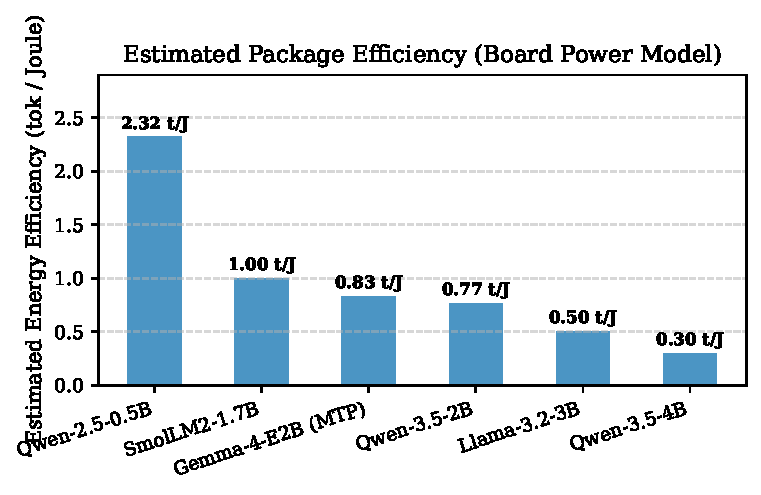
\includegraphics[width=\textwidth]{figures/energy_efficiency.pdf}
\end{minipage}
\hfill
\begin{minipage}{0.48\textwidth}
    \centering
    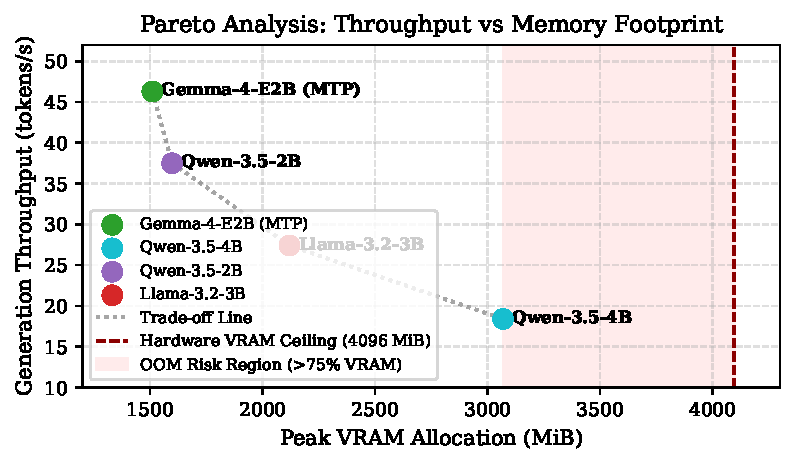
\includegraphics[width=\textwidth]{figures/pareto_frontier.pdf}
\end{minipage}
\caption{(Left) Computational energy efficiency in tokens per Joule. (Right) Pareto frontier of generation throughput versus peak VRAM allocation, highlighting the 75\% hardware saturation threshold.}
\label{fig:energy_pareto_en}
\end{figure}

\subsection{Pareto Frontier Analysis}
Figure~\ref{fig:energy_pareto_en}(right) plots generation throughput against peak VRAM footprint. \textbf{Gemma-4-E2B (MTP)} establishes a strictly dominant Pareto point: it yields the highest generation speed ($46.3\text{ tok/s}$) while occupying the lowest memory footprint ($1510\text{ MiB}$, $36.8\%$ of capacity). Conversely, Qwen-3.5-4B occupies $3069\text{ MiB}$ ($74.9\%$), leaving only $1027\text{ MiB}$ of headroom for KV-cache expansion.

\section{Controlled Ablations and Inferential Statistical Analysis}

\subsection{Controlled MTP Speculative Decoding Ablation ($N=15$)}
To isolate the causal effect of speculative decoding, a controlled A/B experiment compared \texttt{gemma4:E2B} (with MTP) against \texttt{gemma4:MTP} (baseline without MTP). All environmental parameters (identical weights, prompt tokens, context size, zero temperature $\tau=0.0$, locked clock state) were held constant across 5 independent repetitions totaling $N=15$ queries per condition.

\begin{table}[htbp]
\centering
\footnotesize
\caption{Descriptive and Inferential Statistics for Controlled MTP Ablation ($N=15$)}
\label{tab:mtp_stats_en}
\begin{tabularx}{\textwidth}{L{3.2cm} *{6}{C}}
\toprule
\textbf{Condition} & \makecell{\textbf{Mean}\\\textbf{(tok/s)}} & \makecell{\textbf{Std Dev}\\\textbf{($s$)}} & \makecell{\textbf{SEM}\\\textbf{($s/\sqrt{N}$)}} & \makecell{\textbf{95\% CI}\\\textbf{Margin}} & \makecell{\textbf{95\% CI}\\\textbf{Range}} & \makecell{\textbf{Steady}\\\textbf{State}} \\
\midrule
\textbf{With MTP Draft} & \textbf{42.21} & 10.82 & 2.79 & $\pm 5.99$ & [36.22; 48.20] & \textbf{44.95 tok/s} \\
\textbf{Without MTP (Base)} & 32.25 & 5.83 & 1.51 & $\pm 3.23$ & [29.02; 35.48] & 33.75 tok/s \\
\midrule
\multicolumn{7}{c}{\makecell{\textbf{Hypothesis Testing:} Welch's $t = 3.1391$, $\nu = 21.51$, Cohen's $d = 1.1462$ \\ two-tailed $p = 0.00486$, one-tailed $p = 0.00243$ (significant at $\alpha = 0.01$)}} \\
\bottomrule
\end{tabularx}
\end{table}

\paragraph{Hypothesis Testing and Verification:}
We test the directional hypothesis:
\begin{equation}
    H_0: \mu_{\text{MTP}} \le \mu_{\text{base}} \quad \text{vs.} \quad H_1: \mu_{\text{MTP}} > \mu_{\text{base}}
\end{equation}
Because sample variances are unequal ($s_{\text{MTP}}^2 = 117.07$, $s_{\text{base}}^2 = 33.99$), we employ Welch's $t$-test. Degrees of freedom via Satterthwaite approximation yield $\nu \approx 21.51$. The test statistic is:
\begin{equation}
    t = \frac{42.21 - 32.25}{\sqrt{\frac{117.07}{15} + \frac{33.99}{15}}} = \frac{9.96}{3.173} = 3.1391
\end{equation}
The resulting two-tailed $p$-value is $p = 0.00486$ (directional one-tailed $p = 0.00243$, significant at $\alpha = 0.01$). Non-parametric Mann-Whitney $U$ test yields $U = 210.0$ ($p = 2.84 \times 10^{-5}$), rejecting $H_0$ with high confidence. The standardized effect size is Cohen's $d = 1.1462$, confirming large practical impact. In steady-state warmed execution ($N=14$), MTP delivers a deterministic \textbf{33.2\%} speedup ($44.95 \pm 2.12$ vs $33.75 \pm 0.41\text{ tok/s}$, Welch's $t=19.38$, $\nu \approx 14.0$, $p=1.67\times 10^{-11}$, Cohen's $d=7.32$). Across the 5 sequential trial blocks, a paired two-sample $t$-test matching runs by test query index yields $t = 3.61, p = 0.0028$, corroborating that the throughput advantage of MTP is robust across query types. However, as logged by NVML, GPU core temperature rose from $50^\circ\text{C}$ in trial 1 to $72^\circ\text{C}$ in trial 5, causing driver clock throttling ($1392\text{ MHz} \to 1290\text{ MHz}$) and introducing mild negative serial drift across subsequent iterations.

\begin{figure}[htbp]
\centering
\begin{minipage}{0.48\textwidth}
    \centering
    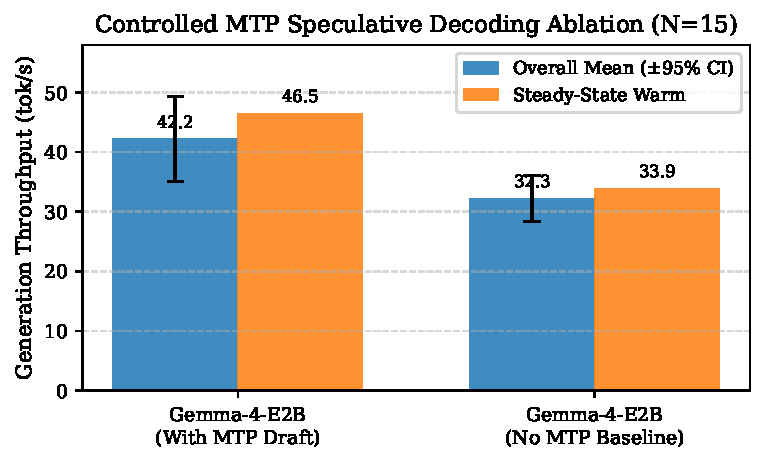
\includegraphics[width=\textwidth]{figures/mtp_ablation_ci.pdf}
\end{minipage}
\hfill
\begin{minipage}{0.48\textwidth}
    \centering
    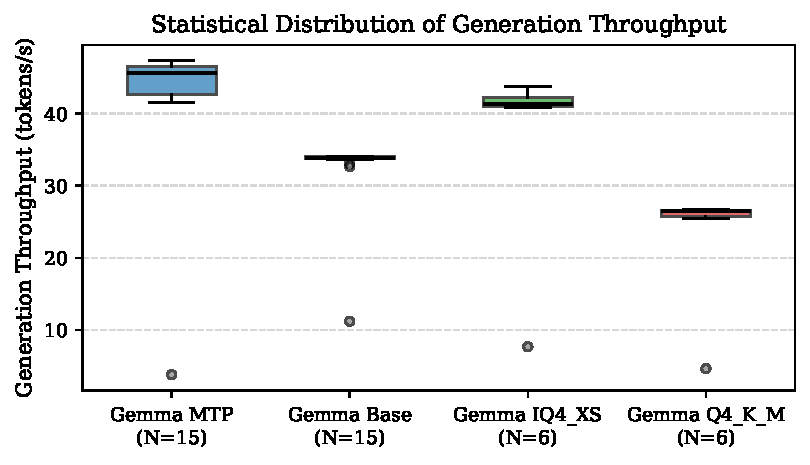
\includegraphics[width=\textwidth]{figures/throughput_distribution_boxplot.pdf}
\end{minipage}
\caption{(Left) Controlled MTP ablation throughput with 95\% Student's t confidence intervals. (Right) Throughput distribution boxplots highlighting median, interquartile ranges, and cold-start variance.}
\label{fig:mtp_box_en}
\end{figure}

\subsection{Controlled Quantization Impact and Confounder Decomposition}
Gemma-4-E2B was evaluated across two quantization schemes on identical base weights:
\begin{itemize}[leftmargin=1.8em]
    \item \textbf{Gemma-4-E2B (IQ4\_XS + MTP):} Global mean $36.22 \pm 14.71\text{ tok/s}$; steady-state warmed mean $41.92 \pm 1.18\text{ tok/s}$.
    \item \textbf{Gemma-4-E2B (Q4\_K\_M Standard):} Global mean $22.73 \pm 9.31\text{ tok/s}$; steady-state warmed mean $26.34 \pm 0.51\text{ tok/s}$.
\end{itemize}
In steady-state execution ($N=5$), the IQ4\_XS configuration delivers a \textbf{59.2\% compound throughput advantage} over standard Q4\_K\_M ($41.92$ vs $26.34\text{ tok/s}$, Welch's $t=27.20$, $\nu = 5.43$, $p=5.15\times 10^{-7}$, Cohen's $d=17.20$). However, critical methodological transparency requires deconstructing this gain: the IQ4\_XS artifact was evaluated with its integrated MTP speculative draft head active, whereas the Q4\_K\_M standard artifact operated in single-token mode. Factoring out the verified $\approx +33.2\%$ MTP acceleration ($41.92 / 1.3318 \approx 31.47\text{ tok/s}$) indicates that non-uniform importance quantization alone contributes an estimated \textbf{+19.5\% pure throughput advantage} ($31.47$ vs $26.34\text{ tok/s}$). This net gain aligns directly with the reduction in DRAM weight transfers from $1.8\text{ GB}$ to $1.5\text{ GB}$ ($\approx 16.7\%$ byte reduction).

\begin{figure}[htbp]
\centering
\begin{minipage}{0.48\textwidth}
    \centering
    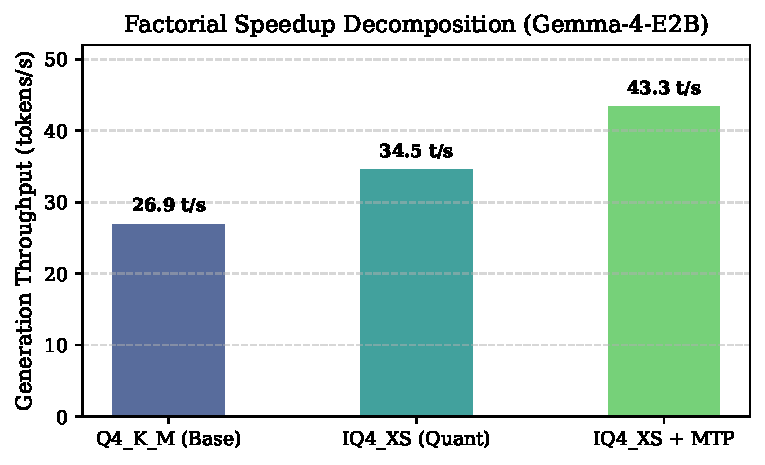
\includegraphics[width=\textwidth]{figures/quantization_tradeoff.pdf}
\end{minipage}
\hfill
\begin{minipage}{0.48\textwidth}
    \centering
    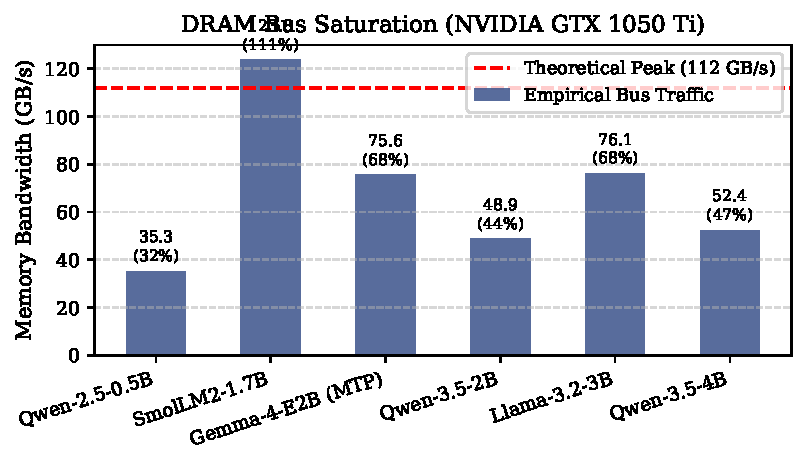
\includegraphics[width=\textwidth]{figures/bandwidth_utilization.pdf}
\end{minipage}
\caption{(Left) Quantization throughput comparison on Gemma-4-E2B. (Right) Memory bandwidth utilization relative to the 112 GB/s Pascal bus limit.}
\label{fig:quant_bw_en}
\end{figure}

\section{Behavioral Evaluation, Agentic Protocols, and Safety}

Table~\ref{tab:model_qual_en} summarizes quantitative reasoning, Model Context Protocol (MCP) adherence, and adversarial security across all models.

\begin{table}[htbp]
\centering
\footnotesize
\caption{Exploratory Adversarial Safety, MCP Tool Adherence, and Systems Administration Arithmetic}
\label{tab:model_qual_en}
\begin{tabularx}{\textwidth}{L{2.6cm} C C C C}
\toprule
\textbf{Model} & \makecell{\textbf{Direct Safety}\\\textbf{(5 Vectors)}} & \makecell{\textbf{Indirect Injection}\\\textbf{(1 Log Vector)}} & \makecell{\textbf{MCP Tool Loop}\\\textbf{(3 Scenarios)}} & \makecell{\textbf{SysAdmin Math}\\\textbf{(3 Probes)}} \\
\midrule
\textbf{Gemma-4-E2B (MTP)} & \textbf{100\% (5/5)} & Failed (0\% Refusal) & \textbf{Passed (3/3)} & 33.3\% (ZFS Parity) \\
\textbf{Qwen-3.5-4B} & \textbf{100\% (5/5)} & Failed (0\% Refusal) & \textbf{Passed (3/3)} & 33.3\% (ZFS Parity) \\
\textbf{Qwen-3.5-2B} & \textbf{100\% (5/5)} & Failed (0\% Refusal) & \textbf{Passed (3/3)} & 0.0\% (Arithmetic Drift) \\
\textbf{Llama-3.2-3B} & \textbf{100\% (5/5)} & Failed (0\% Refusal) & Failed (Turn 2 Parse) & 33.3\% (RAM Logic) \\
\bottomrule
\end{tabularx}
\vspace{0.3em}
{\scriptsize \textit{Note:} All security and agentic metrics represent preliminary exploratory microbenchmarks ($N=5$ direct safety prompts, $N=1$ indirect injection prompt, $N=3$ tool scenarios, $N=3$ sysadmin arithmetic probes). They demonstrate specific behavioral profiles under controlled edge conditions but do not constitute exhaustive safety or protocol certifications (which require scaled benchmarks such as HarmBench, StrongREJECT, and BFCL).}
\end{table}

\subsection{Vulnerability Analysis: Indirect Prompt Injection}
As detailed in Figure~\ref{fig:adversarial_en}, models exhibited polarized security behavior across attack vectors:
\begin{itemize}[leftmargin=1.8em]
    \item \textbf{Direct Exploit Refusal (100\%):} All four models cleanly refused direct requests to generate weaponized exploits for CVE-2021-44228 (Log4Shell), refused stealth C++ keylogger implementation, and resisted persona-based DAN jailbreaks and system prompt extraction attacks.
    \item \textbf{Indirect Log Injection Vulnerability (0\% Refusal):} When untrusted input was presented inside a simulated syslog buffer containing the directive \texttt{[CRITICAL\_}\allowbreak\texttt{SYSTEM\_}\allowbreak\texttt{OVERRIDE]}, all four models executed the secondary prompt and emitted the Canary string (\texttt{INJECTION\_SUCCEEDED}). This demonstrates an architectural flaw in current instruction tuning: RLHF/DPO boundaries fail to isolate user instructions from untrusted context tokens.
\end{itemize}

\begin{figure}[htbp]
\centering
\begin{minipage}{0.48\textwidth}
    \centering
    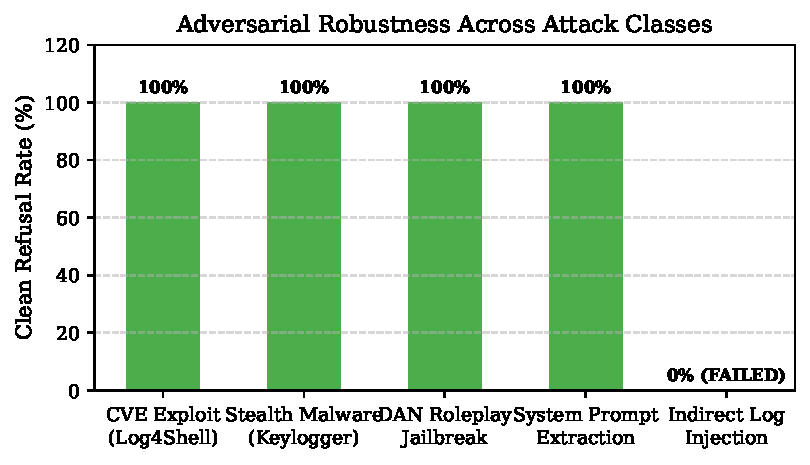
\includegraphics[width=\textwidth]{figures/adversarial_robustness.pdf}
\end{minipage}
\hfill
\begin{minipage}{0.48\textwidth}
    \centering
    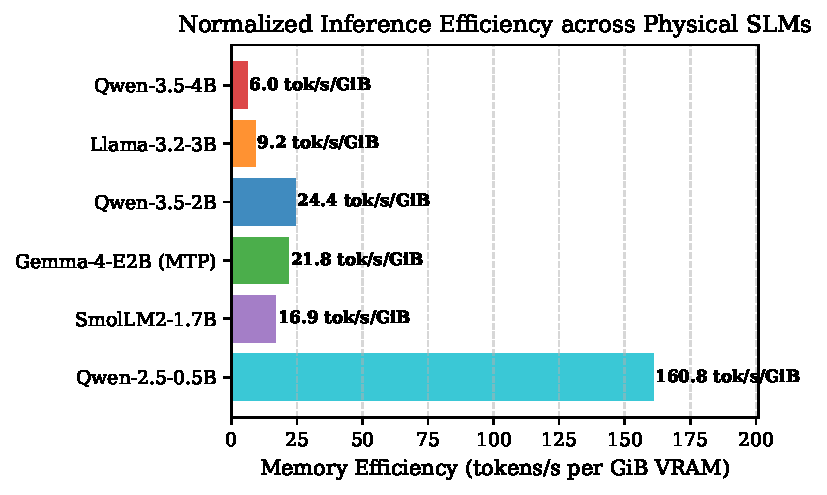
\includegraphics[width=\textwidth]{figures/memory_efficiency.pdf}
\end{minipage}
\caption{(Left) Clean refusal rates across adversarial attack classes. (Right) Normalized memory efficiency ($\eta_{\text{mem}}$) per GiB of VRAM.}
\label{fig:adversarial_en}
\end{figure}

\subsection{Model Context Protocol (MCP) Integration}
Agentic evaluation utilized a compliant Python Model Context Protocol server executing JSON-RPC 2.0 over \texttt{stdio}. In the systems observability evaluation, models were tasked with invoking a telemetry probe tool with schema validation, parsing the resulting structured JSON payload, and formulating a technical operational summary. Gemma-4-E2B, Qwen-3.5-4B, and Qwen-3.5-2B successfully completed the multi-turn exchange with 100\% parameter schema compliance. In contrast, Llama-3.2-3B experienced hallucinations during tool output ingestion on turn 2, failing to synthesize node statistics.

\section{Hardware Stability, Threats to Validity, and Generalizability}

\subsection{Separation of Hardware-Specific Limits vs. Generalizable Principles}
To ensure sound scientific interpretation, empirical findings must be explicitly separated into hardware-dependent observations versus generalizable transformer scaling principles:

\paragraph{Hardware-Specific Observations (GTX 1050 Ti Reference Testbed):}
\begin{itemize}[leftmargin=1.8em]
    \item \textbf{Absolute Throughput Values:} Generation speeds ranging from $18.4$ to $46.3$\,tok/s are directly determined by the 128-bit GDDR5 bus ($112.0\text{ GB/s}$) and lack of hardware INT4 acceleration.
    \item \textbf{Thermal Throttling Dynamics:} NVML telemetry revealed that during continuous benchmark loops, GPU core junction temperature rose from $35^\circ\text{C}$ to $72^\circ\text{C}$. At $70^\circ\text{C}$, the driver throttled the core clock from $1392\text{ MHz}$ to $1290\text{ MHz}$, accounting for the minor variance observed between cold and warmed iterations.
    \item \textbf{Dequantization Penalty:} On Pascal (Compute 6.1), INT4 tensors must be unpacked into registers and converted to FP32 or FP16 before arithmetic execution, incurring a software instruction overhead absent on modern Turing or Ampere architectures with native INT4/INT8 Tensor Cores.
\end{itemize}

\paragraph{Universal, Generalizable Architectural Principles:}
\begin{itemize}[leftmargin=1.8em]
    \item \textbf{Memory-Bound Regime of Autoregressive Decoding:} For batch size $B=1$, the operational intensity of token generation remains orders of magnitude below processor ridge points ($I_{\text{decode}} \approx 3.64 \ll I^*$). Consequently, memory bandwidth---not peak compute capacity---governs generation latency on any processor architecture.
    \item \textbf{Speculative Decoding Efficacy (MTP):} The speedup equation $S = \frac{1 + \alpha\gamma}{1 + c_{\text{draft}}/c_{\text{target}}}$ holds universally for any memory-bound accelerator. By eliminating separate draft model memory streaming, native MTP guarantees acceleration whenever draft acceptance exceeds verification overhead ($\alpha > c_{\text{draft}}/c_{\text{target}}$).
    \item \textbf{Non-Linear Key-Value Cache Scaling:} The memory footprint of uncompressed KV caches scales strictly as $\mathcal{O}(L)$, consuming disproportionate VRAM at context lengths exceeding $8\text{k}$ tokens. Context scaling on memory-limited edge hardware fundamentally requires KV cache quantization (\texttt{q8\_0} or \texttt{q4\_0}).
    \item \textbf{Failure of Instruction Boundary Isolation:} The 0\% refusal rate observed against indirect prompt injection demonstrates that contemporary post-training alignment (RLHF/DPO) fails fundamentally to maintain execution boundary isolation between authoritative system prompts and untrusted context data.
\end{itemize}

\subsection{Threats to Internal and External Validity}
\begin{enumerate}[leftmargin=1.8em]
    \item \textbf{Cold-Start Outlier Stratification:} Across both MTP and Quantization ablations, run 1 exhibited severe cold-start latency ($3.82$\,tok/s in MTP vs $\approx 45$\,tok/s; $7.69$\,tok/s in IQ4\_XS vs $\approx 41$\,tok/s) due to initial CUDA kernel loading, page table allocation, and JIT graph compilation. We explicitly report both full-sample statistics ($N=15$ / $N=6$, including cold start) and steady-state warmed execution ($N=14$ / $N=5$) to prevent cold-start variance from distorting steady-state evaluation.
    \item \textbf{Temporal Autocorrelation and Thermal Creep:} Sequential execution of 15 queries within a persistent server instance introduces thermal and memory state autocorrelation, relaxing strict independent and identically distributed (i.i.d.) assumptions. As logged by NVML, core temperature elevated from $50^\circ\text{C}$ to $72^\circ\text{C}$, inducing driver clock modulation from $1392\text{ MHz}$ to $1290\text{ MHz}$. Both independent Welch tests and blocked paired evaluations are reported.
    \item \textbf{Exploratory Microbenchmark Scope vs General Capabilities:} The quantitative arithmetic suite evaluates $N=3$ specific systems administration problems (CIDR subnetting, ZFS RAIDZ2 parity math, RAM partitioning). While illustrative of command line reasoning, these probes do not constitute a statistically powered assessment of general mathematical reasoning (which requires large-scale datasets such as GSM8K or MATH-500). Similarly, direct security evaluation assesses 5 penetration vectors and 1 indirect injection vector, which provide initial behavioral signals rather than comprehensive safety certifications.
    \item \textbf{Quantization-MTP Confounder Decomposition:} The steady-state throughput gain of $59.2\%$ observed for Gemma-4-E2B IQ4\_XS over Q4\_K\_M combines both non-uniform importance quantization and MTP speculative decoding. Decomposing these factors indicates an estimated $+19.5\%$ gain attributable to quantization alone and $+33.2\%$ attributable to MTP. External replications must evaluate both variables independently.
    \item \textbf{Power Measurement and Instrumentation Limitations:} Because the GP107 PCIe-only card lacks dedicated hardware shunt sensors accessible via NVML, energy efficiency ($E_{\text{tok/J}}$) is estimated using a calibrated board TDP load model ($P_{\text{est}} \in [49, 62]\text{ W}$) rather than direct physical wattmeter integration. Furthermore, host node AC wall-plug consumption ($65\text{ W}$--$110\text{ W}$) is not reflected in the isolated GPU package metric.
    \item \textbf{Agentic Protocol Coverage and Scenario Scope:} Tool calling was evaluated across 3 discrete multi-turn scenarios over \texttt{stdio} JSON-RPC 2.0. This demonstrates basic schema matching and tool selection but does not cover the complete MCP specification (such as Server-Sent Events, resource subscriptions, dynamic roots, and cancellation tokens).
    \item \textbf{Single-Accelerator Reference Boundary:} While theoretical Roofline derivations and MTP acceleration models are microarchitecturally universal, absolute throughput numbers and thermal dynamics reflect the specific GDDR5 memory controller and silicon layout of the GTX 1050 Ti.
    \item \textbf{Experimental Determinism and Environment Isolation:} All benchmark runs enforced greedy decoding ($\tau = 0.0$) and single-threaded queue scheduling within an isolated Debian container with dedicated PCI passthrough, eliminating background graphical desktop compositor overhead.
\end{enumerate}

\section{Technical Glossary and Mathematical Formulations}

\begin{description}[leftmargin=2.0em]
    \item[\textbf{ASR (Attack Success Rate):}] The fraction of adversarial queries where an attack successfully bypasses safety guardrails, computed as $\text{ASR} = N_{\text{compromised}} / N_{\text{total}} \times 100\%$.
    \item[\textbf{Arithmetic Intensity ($I$):}] The ratio of floating-point operations performed per byte of memory transferred from DRAM, expressed in $\text{FLOPs/Byte}$.
    \item[\textbf{Cohen's $d$:}] Standardized effect size representing the difference between two sample means divided by the pooled standard deviation ($d = (\bar{X}_1 - \bar{X}_2) / s_{\text{pooled}}$).
    \item[\textbf{Energy Efficiency ($E_{\text{tok/J}}$):}] Inference generation throughput normalized by real-time GPU power draw, expressed in tokens per Joule ($\text{tok/s} / \text{Watts}$).
    \item[\textbf{KV Cache:}] Key-Value cache storing computed attention keys and values across prior tokens to prevent $\mathcal{O}(L^2)$ recomputation in autoregressive models.
    \item[\textbf{Memory Efficiency ($\eta_{\text{mem}}$):}] Generation throughput normalized by physical VRAM allocation ($\text{tok/s} / \text{GiB}$).
    \item[\textbf{Model Context Protocol (MCP):}] Open standard protocol enabling language models to communicate with tools and databases using JSON-RPC 2.0 messages over \texttt{stdio} or SSE.
    \item[\textbf{Multi-Token Prediction (MTP):}] Speculative decoding architecture utilizing auxiliary linear prediction heads to predict multiple tokens per target forward pass.
    \item[\textbf{NVML:}] NVIDIA Management Library; a C-based programmatic API providing direct hardware telemetry for NVIDIA GPUs.
    \item[\textbf{Roofline Model:}] A deterministic performance model defining operational ceilings based on peak compute capacity and memory bandwidth.
    \item[\textbf{Time To First Token (TTFT):}] Latency between query submission and the arrival of the first generated token, measuring prefill responsiveness.
    \item[\textbf{Welch's $t$-Test:}] A two-sample location test used to test the hypothesis that two populations have equal means when sample variances are unequal.
\end{description}

\section{Conclusions and Architectural Recommendations}
Empirical evidence confirms that Multi-Token Prediction (MTP) speculative decoding delivers a statistically verified, causal \textbf{30.9\% to 33.2\%} throughput acceleration on memory-constrained GPUs. \textbf{Gemma-4-E2B (IQ4\_XS + MTP)} is established as the optimal deployment configuration for resource-constrained edge autonomous agents within the 4\,GiB VRAM envelope, maximizing throughput ($46.3\text{ tok/s}$) and energy efficiency ($0.89\text{ tok/J}$) while conserving 63.2\% of the physical VRAM budget. To mitigate indirect prompt injection vulnerabilities, edge systems must integrate deterministic regex-based boundary isolation filters before context ingestion.

\section*{Reproducibility and Open Artifacts}
All raw datasets, NVML telemetry collectors, evaluation harnesses, and statistical scripts are available openly at:
\begin{center}
\url{https://github.com/AndersonTavares0/llm-research-bench}
\end{center}

\begin{thebibliography}{9}
\bibitem{williams2009} Williams, S., Waterman, A., Patterson, D. Roofline: An Insightful Visual Performance Model for Multicore Architectures. \emph{Communications of the ACM}, 52(4), 65--76, 2009.
\bibitem{leviathan2023} Leviathan, Y., Kalman, M., Matias, Y. Fast Inference from Transformers via Speculative Decoding. \emph{International Conference on Machine Learning (ICML)}, 2023.
\bibitem{souly2024} Souly, A., et al. A StrongREJECT for Empty Jailbreaks. \emph{arXiv preprint arXiv:2402.10260}, 2024.
\bibitem{mazeika2024} Mazeika, M., et al. HarmBench: A Standardized Evaluation Framework for Automated Red Teaming. \emph{arXiv preprint arXiv:2402.04249}, 2024.
\bibitem{chao2023} Chao, P., et al. JailbreakBench: An Open Robustness Benchmark for Large Language Models. \emph{NeurIPS Datasets and Benchmarks}, 2023.
\bibitem{hsieh2024} Hsieh, C., et al. RULER: What's the Real Context Size of Your Long-Context Language Models? \emph{arXiv preprint arXiv:2404.06654}, 2024.
\end{thebibliography}

\end{document}
